%**********************************************************
The remote system is responsible for the communication between the local systems and the internet. In this project, the internet is used to maintain a cloud database, so the remote system does the data bridge between the network of street lampposts and a cloud. As one can see in figure \ref{fig:rs_overview}, the remote system is composed by the main process and a daemon process \textit{dServerSend}. The main process may be composed of a server and varoius clients, being the messages from each client received and processed in this process. The messages are sent to the clients in the daemon process \textit{dServerSend}. The communication between the two processes is done using message queues, so when a command is received and successfully parsed, the main process sends the command output to the daemon using the message queue.

\begin{figure}[H]
	\centering
	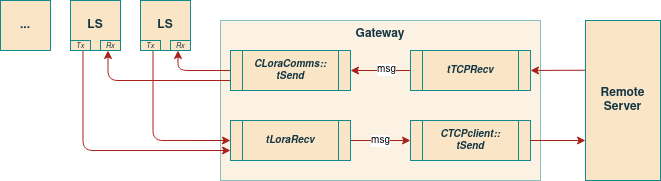
\includegraphics[width=.6\textwidth]{09sw_specification/RS/overview}
	\caption{Inter-process Communication between Main Process and Daemon.}
	\label{fig:rs_overview}
\end{figure}

%**********************************************************
\subsection{Class Diagram}
In figure \ref{fig:rs_classDiag} is represented the class diagram of the remote system. The class \textit{CTCPServer} is the main class of the system, that initializes the objects of each class, listed below. 

\begin{itemize}
	\item \textbf{CTCPServer:} main class, responsible for creating the server, the client objects, each time a client connects to the server and for sending the messages to the clients;
	\item \textbf{CClient:} client class, stores the clients information and receives their messages;
	\item \textbf{CDataBase:} provides an interface between the server and the database.

\end{itemize}

\begin{figure}[H]
	\centering
	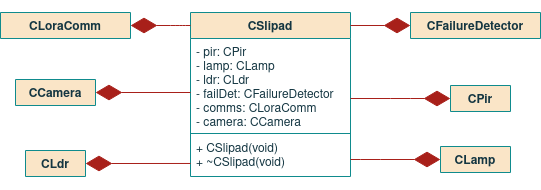
\includegraphics[width=.9\textwidth]{09sw_specification/RS/ClassDiagram}
	\caption{Remote System Class Diagram.}
	\label{fig:rs_classDiag}
\end{figure}

%****************************
\myparagraph{Class CTCPServer}

This class is responsible for creating the server, using \textit{createServer} function, allowing multiple clients to connect and send them messages, with the thread \textit{tSend}. When a client connects to the server, this class creates a new instance of the class \textit{CClient}. Each client can be of a different type of device like website, mobile application or gateway. The clients are assigned to their respective list of clients that are \textit{webSList}, \textit{appList} and \textit{gatewayList}, respectively. To do the interface with the database, this class also has an instance of the class database. In figure \ref{fig:CTCPServer}, one can see the class \textit{CTCPServer} diagram.

\begin{figure}[H]
	\centering
	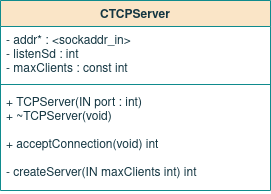
\includegraphics[width=.6\textwidth]{09sw_specification/RS/CTCPServer/CTCPServer}
	\caption{Class Diagram: CTCPServer.}
	\label{fig:CTCPServer}
\end{figure}

%****************************
\myparagraph{Class CClient}

The class \textit{CClient}, represented in figure \ref{fig:CClient}, is responsible for storing information about a client connected to the server, like the \textit{cmdList}, a vector that stores all the client commands list and \textit{clientSock}, and also for receiving messages from the clients in the thread \textit{tRecv}. The \textit{clientSock} has information about the client connected such as its \textit{state}, its client identification (\textit{index}), its name in \textit{clientName}, its file descriptor \textit{sockFd} and its type of client \textit{type}, that can be: \textit{GATEWAY}; \textit{WEBSITE}; or \textit{APPLICATION}.

\begin{figure}[H]
	\centering
	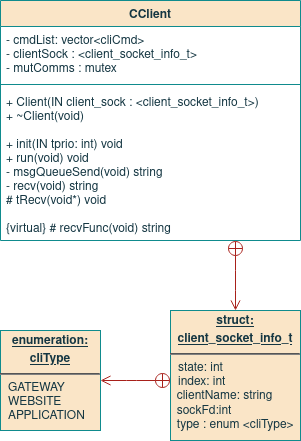
\includegraphics[width=.6\textwidth]{09sw_specification/RS/CClient/CClient}
	\caption{Class Diagram: CClient.}
	\label{fig:CClient}
\end{figure}

%****************************
\myparagraph{Class CDataBase}

This class diagram is shown in figure \ref{fig:CDataBase}, and is responsible for implement the interface between the server and the database, having for that a pointer to a database of type \textit{MYSQL}. To interact with the database, the server must first prepare a query, using the function \textit{prepareQuery}, and can update or get data from the database, using the prepared query and the functions \textit{updateData} and \textit{getData}, respectively.

\begin{figure}[H]
	\centering
	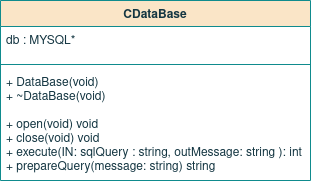
\includegraphics[width=.5\textwidth]{09sw_specification/RS/CDataBase}
	\caption{Class Diagram: CDataBase.}
	\label{fig:CDataBase}
\end{figure}

%**********************************************************
\subsection{Task Overview}
One can define and describe briefly how the remote system is implemented, making use of threads and processes. 

\begin{itemize}
	\item \textbf{tSend:} sends a message to a client;
	\item \textbf{tRecv:} receives a message from the clients.
\end{itemize}

%**********************************************************
\subsection{Task Priority}
As the two threads \textit{tRecv} and \textit{tSend} run in two different processes, daemon process and main process, respectively, one needs to define the threads priority assignment for the two processes. The priority assignment diagram for the remote system main process is represented in figure \ref{fig:rsMainPrio} and for the daemon process is shown in the figure \ref{fig:rsDaemonPrio}. 

\begin{figure}[H]
	\centering
	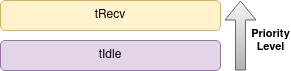
\includegraphics[width=.5\textwidth]{09sw_specification/RS/MainPrio}
	\caption{Remote System Main Process Priority Assignment.}
	\label{fig:rsMainPrio}
\end{figure}

\begin{figure}[H]
	\centering
	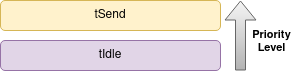
\includegraphics[width=.5\textwidth]{09sw_specification/RS/DaemonPrio}
	\caption{Remote System Daemon Process Priority Assignment.}
	\label{fig:rsDaemonPrio}
\end{figure}

%**********************************************************
\subsection{Task Synchronization}
As seen before, to have coordinate access to shared ressouces and services and avoid race conditions, the kernel has resources that provide synchronization between the tasks. 

\myparagraph{Mutexes}

The mutexes used for the remote system are listed bellow.

\begin{itemize}
	\item \textbf{CTCPServer::mutComms:} mutex used to protect the messages sending;
	\item \textbf{CClient::mutComms:} mutex used to protect the messages receiving.
\end{itemize}

\subsection{Task Communication}
\myparagraph{Message Queues}

In order to the main process communicate with the daemon process and send messages to the clients, one can use a message queue, named \textit{msgqComms}, that send the messages from the main process to the daemon process, containing the messages to be sent from the server to the clients.

%**********************************************************
\subsection{Flowcharts}
\myparagraph{CTCPServer}

In figure \ref{fig:ServerConst} is represented the constructor of the \textit{CTPCServer} class, that is responsible for creating the class variables, initializing the mutex and for creating the thread \textit{tSend} and the server socket in the port passed by argument.

\begin{figure}[H]
	\centering
	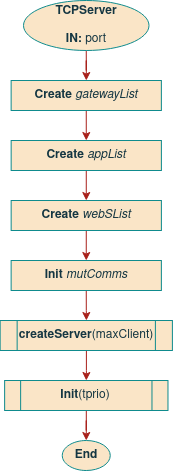
\includegraphics[width=.26\textwidth]{09sw_specification/RS/CTCPServer/ServerConst}
	\caption{Flowchart: CTCPServer Constructor.}
	\label{fig:ServerConst}
\end{figure}

The function that creates a server socket for a maximum number of clients, \textit{maxClient}, is represented in figure \ref{fig:RSCreateServer}. This function initiates a server socket with the IPv4 protocol connection.

\begin{figure}[H]
	\centering
	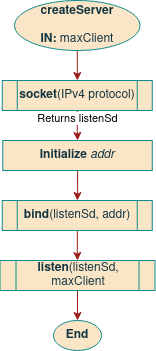
\includegraphics[width=.3\textwidth]{09sw_specification/RS/CTCPServer/CreateServer}
	\caption{Flowchart: CTCPServer createServer.}
	\label{fig:RSCreateServer}
\end{figure}

In figure \ref{fig:RSInit}, is shown the method that creates the thread \textit{tSend} with the priority \textit{tprio} passed by argument.

\begin{figure}[H]
	\centering
	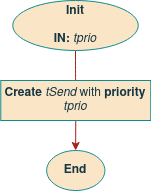
\includegraphics[width=.26\textwidth]{09sw_specification/RS/CTCPServer/Init}
	\caption{Flowchart: CTCPServer Init.}
	\label{fig:RSInit}
\end{figure}

The function \textit{run} is responsible for waiting for the termination of the thread \textit{tSend}.

\begin{figure}[H]
	\centering
	\includegraphics[width=.26\textwidth]{09sw_specification/RS/CTCPServer/run}
	\caption{Flowchart: CTCPServer run.}
	\label{fig:RSrun}
\end{figure}

In figure \ref{fig:RSsend} is represented the thread \textit{tSend}, which is responsible for sending a message to a client. It reads the messages to be sent in a message queue and send them to the recipient client.

\begin{figure}[H]
	\centering
	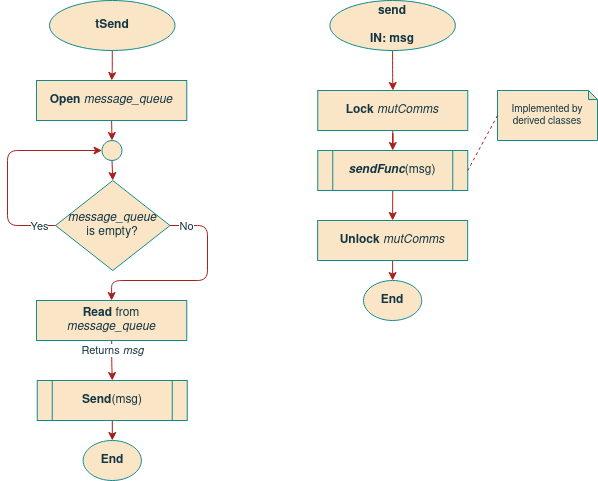
\includegraphics[width=.95\textwidth]{09sw_specification/RS/CTCPServer/send}
	\caption{Flowchart: CTCPServer tSend.}
	\label{fig:RSsend}
\end{figure}

%**********************************
\myparagraph{CClient}

In figure \ref{fig:ClientConst} is represented the constructor of the \textit{CClient} class. Every time a client connects to the server, it creates an instance of this class, passing by argument, the information about the client to initialize the \textit{clientSock} variable. The constructor also creates the command list that the type of client can execute, \textit{cmdList}, and the thread \textit{tRecv}.

\begin{figure}[H]
	\centering
	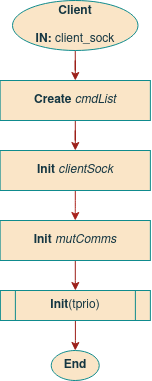
\includegraphics[width=.20\textwidth]{09sw_specification/RS/CClient/ConsClient}
	\caption{Flowchart: CClient Constructor.}
	\label{fig:ClientConst}
\end{figure}

The command list, \textit{cmdList} varies with the type of client:

\begin{itemize}
	\item \textbf{Mobile Application:} 
		\begin{itemize}
			\item Get;
			\item Update;
			\item Delete.
		\end{itemize}
	
	\item \textbf{Web Site:}
		\begin{itemize}
			\item Get.			
		\end{itemize}
	
	\item \textbf{Gateway:}
		\begin{itemize}
			\item Get;
			\item Update.
		\end{itemize}

\end{itemize}

In the method \textit{init}, shown in figure \ref{fig:clientInit}, it is created the thread \textit{tRecv}, that receives messages from the clients, with priority \textit{tprio}.

\begin{figure}[H]
	\centering
	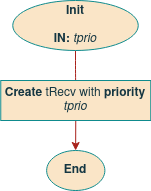
\includegraphics[width=0.3\textwidth]{09sw_specification/RS/CClient/init}
	\caption{Flowchart: CClient Init.}
	\label{fig:clientInit}
\end{figure}

The method \textit{run}, represented in figure \ref{fig:clientRun}, is responsible for waiting for the termination of the thread \textit{tRecv}.

\begin{figure}[H]
	\centering
	\includegraphics[width=0.3\textwidth]{09sw_specification/RS/CClient/run}
	\caption{Flowchart: CClient Run.}
	\label{fig:clientRun}
\end{figure}

The figure \ref{fig:RSRecv} shows the thread that receive messages from the clients, \textit{tRecv}. When a message is received, the function \textit{recvFunc} returns the message. If the message is not empty, then one can parse and execute a command extracted from the message sent, using the \textit{parseExecute} function. When the command is valid, this function returns a message to be sent back to the client. As the send thread belongs to a daemon, one can send the message to the daemon process using a message queue.

\begin{figure}[H]
	\centering
	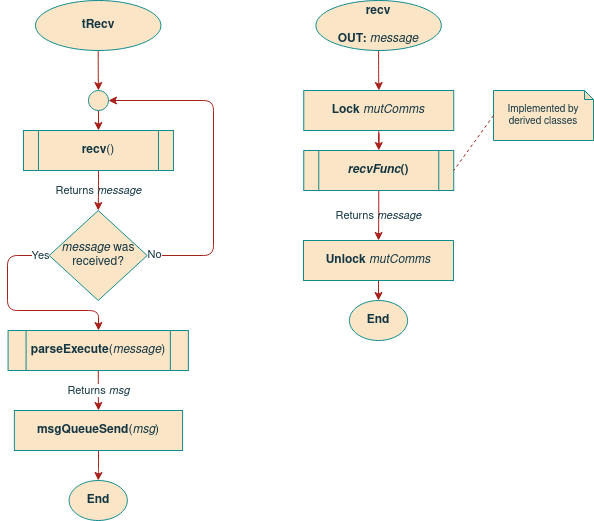
\includegraphics[width=0.95\textwidth]{09sw_specification/RS/CClient/recv}
	\caption{Flowchart: CClient tRecv.}
	\label{fig:RSRecv}
\end{figure}

In figure \ref{fig:parseExecute} is represented the flowchart of the \textit{parseExecute} function, that is responsible for parsing and execute the message sent by the client. It is needed to verify if the client that sent the command has rights to execute that command, so the message sent is searched in the \textit{cmdList} assigned to the respective client. If the message corresponds to a valid command for that client, then one can prepare a query and execute the command according to the type of command that was sent: \textit{delete} for a data deletion, \textit{update} for a data update and \textit{get} for a data request, returning the command output in a string message \textit{msg}. If the command doesn't exist in the command list of that client, then the \textit{msg} is assigned with an error message. The output of this function is the string message, \textit{msg}.

\begin{figure}[H]
	\centering
	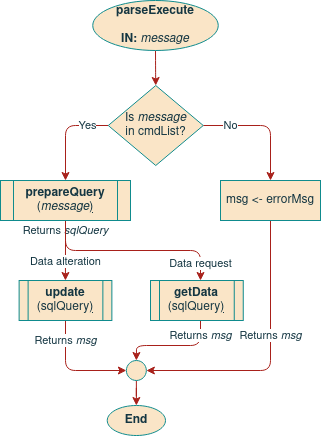
\includegraphics[width=0.95\textwidth]{09sw_specification/RS/CClient/parseExecute}
	\caption{Flowchart: CClient parseExecute.}
	\label{fig:parseExecute}
\end{figure}

%**********************************************************
\subsection{Start-up Process}
The start-up process is shown in the figure \ref{fig:RSstart}. When the program initiates, the start-up process instantiate a object of the class \textit{CTCPServer}. After that, it waits for the thread to terminate, using the function \textit{run}.

\begin{figure}[H]
	\centering
	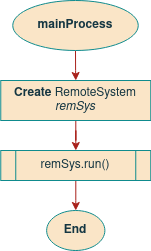
\includegraphics[width=0.3\textwidth]{09sw_specification/RS/CClient/start}
	\caption{Start-Up Process.}
	\label{fig:RSstart}
\end{figure}